\chapter{Documents, Hypertext and MHEG}

\section{Document Architecture and Multimedia Integration}
Document is a set of structured information which may be present in various media and may be generated or input at the time of presentation. A document is used by humans and is available for editing in a computer.

\subsection*{Documents}
\begin{itemize}
	\item A \emph{multimedia document} is characterized by information which is coded in at least one continuous (time-dependent) and one discrete (time-independent) medium. \item The integration of various media is possible because of close relationships between information units. 
	\item This is also called \emph{synchronization}. 
	\item A multimedia document should be viewed in the environment of tools, data abstractions, basic concepts, and document architectures.
	
\end{itemize}

%Continuous and discrete data are still viewed and treated in many different ways. A text within an editing program is treated as a type of programming language (type character), and a motion picture is manipulated in the same editing program only via library calls. The levels of view are different, and so are the manipulation options. The goal of abstraction of multimedia data is an integrated, uniform way of describing and handling all media. This means an essential reduction of the complexity with regard to setting up and maintaining such programs. Abstractions of multimedia data serve as a basis for writing code for many different types of multimedia programs, in particular editors and other document processing tools.


Fundamental system concepts use abstractions of multimedia data, they serve as a concept for information architectures, and they can be implemented by use of tools. In this respect, the terms \textit{document architecture} and \textit{information architecture} are synonymous.


\subsection{Document Architecture}
\begin{itemize}
	\item Exchange of documents means the communication of both content and structure. 
	\item In addition to common communication protocols, it also requires the use of a document architecture. 
	\item This includes standardized architectures, such as SGML (Standard Generalized Markup Language).
	\item Such information architectures use data abstractions and their concepts for specification and implementation. 
	\item A document architecture describes the interplay of models (see Figure {\ref{fig:document-arch}}).
\end{itemize}


Figure {\ref{fig:document-arch-component}} shows a multimedia information architecture characterized by the internal interplay of individual information units from discrete and continuous media.


In the interplay of models, the manipulation describes operations that can be performed on multimedia information. 
\begin{itemize}
	\item \textit{Communication} and \textit{storage} define the protocols used to exchange this information between different computers and the format used to store data.
	\item The \textit{presentation} of multimedia information collects relationships between individual parts of information, which have to be maintained in the presentation of this information. 
\end{itemize}

Not every architecture includes all properties or models mentioned here.




%%%%%%%%%%%%%%%%%%%%%%%%%%%%%%%%%%%%%%%%%
%										%
%				FIGURE				   	%
%										%
%%%%%%%%%%%%%%%%%%%%%%%%%%%%%%%%%%%%%%%%%
\begin{figure}[ht!]
	\centering
	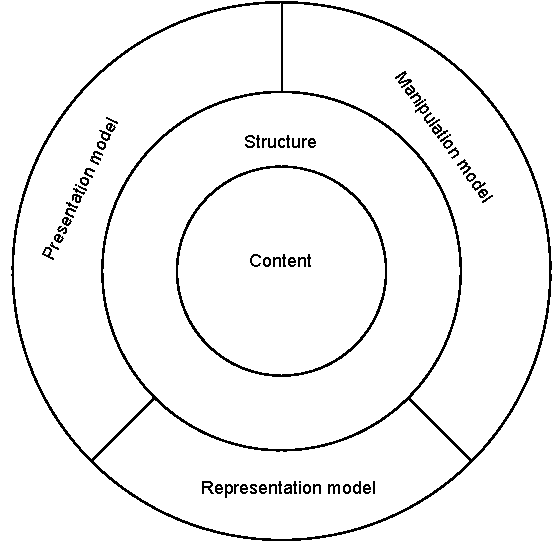
\includegraphics[width=0.6\textwidth]{document-arch}
	\caption{Architecture of documents and their components.}{\label{fig:document-arch}}
\end{figure}
%--------------------------Figure end -------------------

%%%%%%%%%%%%%%%%%%%%%%%%%%%%%%%%%%%%%%%%%
%										%
%				FIGURE				   	%
%										%
%%%%%%%%%%%%%%%%%%%%%%%%%%%%%%%%%%%%%%%%%
\begin{figure}[hb!]
	\centering
	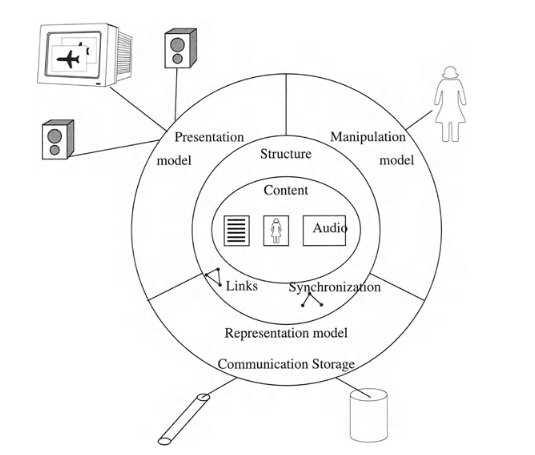
\includegraphics[width=0.8\textwidth]{document-arch-components}
	\caption{Architecture of multimedia documents and their components.}{\label{fig:document-arch-component}}
\end{figure}
%--------------------------Figure end -------------------


\subsection{Multimedia Integration}
See Section \ref{sec:notion-of-synchronization}, Page No.\ \pageref{sec:notion-of-synchronization}.
\section{Hypertext, Hypermedia and Multimedia}
A book or an article in paper form has a pre-determined structure and is present in sequential form. However, we can read specific sections in a targeted way without having read previous sections. Authors normally assume sequential reading, so that many sections are based on knowledge previously acquired. Both fictional literature and movies always assume a purely sequential reception. Scientific literature can consist of independent chapters. However, in this context too, sequential reading is assumed.


Technical documentation (e.\ g.\, manuals) consists often of a collection of relatively independent information units. A lexicon or reference book about the Airbus, for example, is generated by several authors and always only parts are read sequentially. There also exist many cross-references in such documentations which lead to
multiple searches at different places for the reader. Here, an electronic help facility, consisting of information links, can be very significant.

Figure \ref{fig:hypertext-data} shows an example of such a concatenation or linking. 

\begin{figure}[ht!]
	\centering
	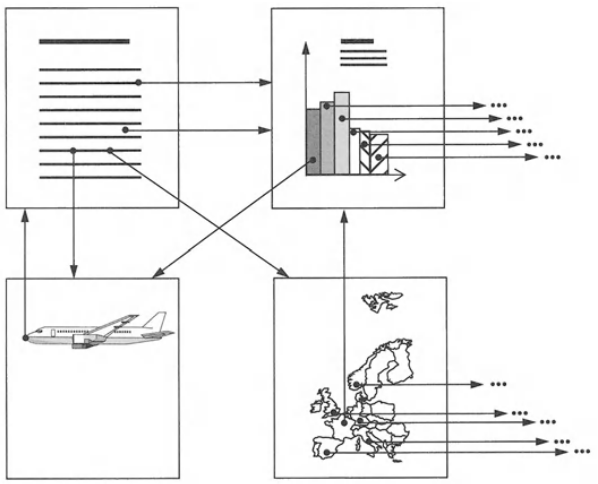
\includegraphics[width=0.7\textwidth]{hypertext-data}
	\caption[Hypertext data.]{Hypertext data. An example of linking information of different media.}
	\label{fig:hypertext-data}
\end{figure}

\begin{multicols}{2}
\begin{enumerate}
	\item Each arrow specifies a relationship between logical information units (LDUs). 
	\item A piece of text (top left in the figure) includes a reference to the climb properties of an aircraft. 
	\item These properties are demonstrated in a video sequence (bottom left in the figure). 
	\item At a different location in the same text, the sales subsidiaries located in Europe are listed (and the list is visualized in a graphical map, shown at the bottom right in the figure).
	\item More information about each sales point can be viewed by selecting that location in the graphical	map. 
	\item A special piece of information about the number of different aircrafts sold in the Paris subsidiary is shown in the form of a bar chart (top right in the figure). \item Internally, all information contained in this chart are present only in tabular form. 
	\item The left bar refers to the aircraft, which can be seen in a video.
\end{enumerate}

\end{multicols}


\subsection*{Non-linear Linking of Information}
\begin{multicols}{2}
	\begin{enumerate}
	\item The most important property of hypertext and hypermedia is non-linear information linking. 
	\item There is a reading sequence, but the reader also decides about the reading path. 
	\item For example, when browsing in a lexicon, the reader can start with the term hypertext and then use the cross-reference systems to jump to a description of AppleTalk. 
	\item Using this association, based on reference links, the	author of the information normally determines the links.
	\end{enumerate}
\end{multicols}


A hypertext structure is a \textit{graph}, consisting of \textit{nodes} and \textit{edges}.
\begin{multicols}{2}
	\begin{enumerate}[label=(\alph*)]
		\item The \textit{nodes} are the actual information units. 
		\item They are, for example, the text elements, individual graphics, audio or video LDUs. 
		\item The \textit{edges} form a relationship between different information units. They are called \textit{reference} or \textit{link}. 
		\item A reference is normally a directed edge. 
		\item All linking elements contain information.
	\end{enumerate}
\end{multicols}

Figure {\ref{fig:hyper-multi}} shows the relationship between multimedia, hypertext, and hypermedia.

%%%%%%%%%%%%%%%%%%%%%%%%%%%%%%%%%%%%%%%%%
%										%
%				FIGURE				   	%
%										%
%%%%%%%%%%%%%%%%%%%%%%%%%%%%%%%%%%%%%%%%%
\begin{figure}[ht!]
	\centering
	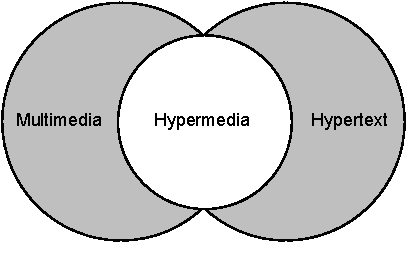
\includegraphics[width=0.5\textwidth]{hyper-multi}
	\caption{Hypertext, hypermedia and multimedia, and their relationships.}{\label{fig:hyper-multi}}
\end{figure}
%--------------------------Figure end -------------------


\subsection[Hypertext]{Hypertext System}
\begin{multicols}{2}
	\begin{itemize}
		\item A hypertext system is essentially characterized by non-linear linkage of information. 
		\item Pointers/References connect the nodes. 
		\item The data of various nodes can be present in one medium or several media. 
		\item In a pure text system, only the text sections are	linked. 
		\item The term \textit{hypertext} means that several media can be linked, in addition to simple	text.
	\end{itemize}
\end{multicols}


\subsection[Multimedia]{Multimedia System}
\begin{multicols}{2}
	\begin{itemize}
		\item A multimedia system contains information encoded at least in one continuous and one discrete medium. 
		\item For example, when text data are connected by a non-linear link, then this belongs to the hypertext category. 
		\item A video conference with simultaneous transmission of text and graphics from a conventional linear program for document editing is a multimedia application.
	\end{itemize}
\end{multicols}


\subsection[Hypermedia]{Hypermedia System}
\begin{multicols}{2}
	\begin{itemize}
		\item A hypermedia system includes the non-linear linkage of information which is normally present in either a continuous or a discrete medium. 
		\item For example, text and video data within a non-linear linkage structure belong to the hypermedia, multimedia, and hypertext categories.
	\end{itemize}
\end{multicols}



Figure {\ref{fig:hyper-multi}} shows that each hypermedia system belongs to the hypertext category and is a multimedia system at the same time. It forms the intersection set of both multimedia and hypertext.

\subsubsection*{Application Areas of of Hypermedia}
\begin{multicols}{2}
	\begin{itemize}
		\item \textit{Computer-based applications} to include the help function of modern graphical interface.
		\item \textit{Commercial applications} include repair and operating instructions.
		\item \textit{Intellectual applications} include organization of ideas, brainstorming, or text creation.
		\item \textit{Education and research} are areas with a large potential for improvement by use of continuous media.
		\item The \textit{entertainment industry} has used hypertext for information or guiding systems for tourists and interactive science-fiction movies.
	\end{itemize}
\end{multicols}


\section{Systems: Architecture, Nodes and Pointers}

\subsection{Architecture}
The architecture of a hypertext system can be divided into \textit{three levels} with different functionalities.
%\begin{center}
%	\begin{framed}
%			\begin{nepali}
%			\textbf{नाेट}: याे शीर्षक भित्र level अथवा layer भनेमा एउटै हुन् भन्ने बुझिन्छ। अरुकाे नाेटमा layer लेखेकाे भएपनि दुवै एकै हाे भनेर मान्ने।
%		\end{nepali}
%	\end{framed}
%%	%\end{center}

\begin{multicols}{2}
	\begin{enumerate}
		\item \textit{Presentation Level}
		\item \textit{Hypertext Abstract Machine} 
		\item \textit{Storage/Databse Level}
	\end{enumerate}
\end{multicols}

\subsubsection[Presentation Level]{Top Level: Presentation Level}
\begin{multicols}{2}
	\begin{itemize}
		\item The top or \textit{presentation level} accommodates all functions relating to the user interface. 
		\item This level is used to map nodes and references to the user interface. 
		\item The user interface offers the visualization of one or several sections. 
		\item This level determines the data to be displayed and how it should be represented based on the structure and the display chosen by the user.
		\item This level is also responsible for the control of all inputs.
	\end{itemize}
\end{multicols}


\subsubsection[Hypertext Abstract Machine]{Hypertext Abstract Machine (HAM)}
\begin{multicols}{2}
	\begin{itemize}
		\item The HAM is located between the presentation level (level One) and the storage level (level Two).
		\item This level takes database-like functions to store multimedia data within a local or distributed environment from the lower level. 
		\item HAM level does not have to worry about the input and output of the upper level. 
		\item HAM knows the structure of a document, and it disposes of knowledge about the references and their attributes. 
		\item This means that the HAM level builds the data structure, or an object hierarchy, for document management. 
	\end{itemize}
\end{multicols}

Compared to the other two levels, the HAM level is the one least dependent on the system. This means that it is also best suitable for standardization.

\subsubsection[Storage Level]{Storage/Database Level}
\begin{multicols}{2}
\begin{itemize}
	\item The \textit{storage level} (also called \textit{database level}) forms the lowest level. 
	\item It includes all functions relating to the storage of data, i.\ e.\ , secondary storage management. 
	\item In this respect, the specific properties of the different sets of data from discrete and continuous media are important. 
	\item This is also the level where capabilities of traditional database systems, i.\ e.\ , persistence, multi-user operation
	(synchronization, locking), and error recovery (transaction concept), are expected. 
	\item The nodes and pointers of a hypertext document are processed as data objects without any special semantics.
\end{itemize}
\end{multicols}



\noindent Unfortunately, most implementations of hypertext systems do not clearly separate these different levels. The reasons are normally a shorter development phase, a more efficient implementation, and shortcomings in most generally available multimedia interfaces for the lowest level.

\subsection{Nodes}
A node is an information unit (LDU) in a hypertext document. The most important distinguishing criterion between different implementations is the maximum data quantity a node can accommodate.

\subsubsection{Maximum Data Quantity}

\begin{multicols}{2}
	\begin{itemize}
		\item The \textit{maximum data quantity} contained in a node can be limited to match the screen size.
		\item A motion picture sequence and an audio clip could be limited to a duration of, for example, 36 seconds.
	\end{itemize}
\end{multicols}
An author is forced eventually to distribute logical connected text content to several cards, although it is not desired. Applying it to video clips and audio passages, it would mean that the close interconnection among the distributed sequences could get lost easily. An advantage is the \textit{clear and intuitive environment}.


\subsubsection{Unlimited Data Quantity}
\begin{multicols}{2}
	\begin{itemize}
		\item One alternative are window-based systems with a basically \textit{unlimited data quantity} per node. 
		\item Forward and backward scrolling of pages is offered analogous to other windows at the user interface. 
		\item \textit{Intermedia} is such a system. Intermedia does not limit the duration of continuous media with regard to the data volume its nodes can accommodate.
	\end{itemize}
\end{multicols}

This means that single nodes can have very different lengths and still appear equal-ranking. The presentation of additional information also uses two different methods at the user interface: 

	\begin{itemize}
			\item First, there is a way to switch between the nodes,
			\item and second, a node uses the mechanisms known from window-based systems for \textit{scrolling}.
	\end{itemize}

	

\noindent A secondary criterion concerns the \textit{time when a piece of information is created}. In general, the author can specify the entire contents of the nodes while creating a document.

\subsection{Pointers}
%\begin{center}
%	\begin{framed}
%	\begin{nepali}
%		नाेटः यस शीर्षक भित्र pointer अथवा reference भन्नु एउटै हाे।
%	\end{nepali}
%	\end{framed}
%\end{center}
\textit{Pointers/References} form the edges in a hypertext graph. Hypertext systems differ by various edge criteria. One of the first questions to ask here would be: \textit{Which information is contained in a pointer?}

\begin{multicols}{2}
	\begin{itemize}
		\item \textit{Simple pointers} connect two nodes of a graph without containing any information themselves. They merely establish a relationship between those nodes.
		
		\item \textit{Typified pointers} connect two nodes and include additional information. A label is assigned to each reference. This label is used to create comments to each reference (e.\ g.\ , author and creation date).
	\end{itemize}
\end{multicols}


Another Property of the pointers is connected to the question: \textit{What does the pointer mean?} Often, pointers with very different meanings are used together. This usage complicates the understanding. The author of a hypertext should know about this problem and use unambiguous pointers. The following relations can be expressed through pointers:

\begin{multicols}{2}
	\begin{itemize}
		\item \textit{To be} - $ A $ is part of $ B $. This represents a quantity relationship.
		\item \textit{To present} - $ A $ is an example of $ B $, or $ A $ demonstrates $ B $. This case uses an example to state a fact.
		\item \textit{To produce} - $ A $ produces $ B $, or $ B $ is a result of $ A $. This case can describe consequences from a fact in more detail.
		\item \textit{To require or required by} - $ A $ requires $ B $, $ B $ needs $ A $. This relationship expresses
		an absolute necessity.
		\item \textit{To own} - $ A $ owns $ B $, or $ A $ is associated to $ B $. This relationship expresses an ownership.
		\item \textit{To include} - $ A $ includes $ B $, or $ A $ consists of $ B $, or $ A $ occurs in $ B $. This relationship
		represents different meanings of an inclusion.
		\item \textit{Similarity} - $ A $ is similar to $ B $, $ A $ is different from $ B $, $ A $ replaces $ B $, $ A $ is the alternative to $ B $. This relationship expresses similarities.
	\end{itemize}
	
\end{multicols}

Another fundamental property of pointers can be described by the following question: \textit{Who states a pointer?} We distinguish as follows:
\begin{multicols}{2}
	\begin{itemize}
		\item \textit{Implicit References}: A relationship between nodes can be created automatically by a hypertext system. The author specifies only the algorithms used to create the references. 
		
		\item \textit{Explicit References}: All references are created by the author.
	\end{itemize}
\end{multicols}


A reference can be created at different times, which leads us to the question: \textit{When is the target of a pointer stated?}

\begin{multicols}{2}
	\begin{itemize}
		\item In the classical case, a reference is created during the creation of the hypertext document, and both the origin and the target node are specified. When editing the	document, the author specifies explicitly how the information units should be
		linked.
		
		\item A target node can be determined when the reference is used, i.\ e.\ , while the document is read. The author specifies an algorithm to be used to create the references, while the references are determined when the user reads the context. The system 	calculates the target node.
	\end{itemize}
\end{multicols}

In most systems, however, each pointer has exactly one origin and one target node. On the other hand, we could ask the following question:
\begin{itemize}
	\item \textit{ What direction does the pointer have?} and
	\item \textit{What is the number of outgoing pointers?}
\end{itemize}


\begin{multicols}{2}
	\begin{itemize}
		\item The direction is normally unidirectional, while the system itself supports \textit{backtracking}. This means that we would always get back on track.
		\item The alternative would be bidirectional references, which means that we would have to highlight or mark both the target nodes and the anchors. When introducing bidirectional references, it could easily happen that several nodes refer to the same target nodes. This means that these references have to be explicitly distinguished at the target node.
		\item The same applies to references leading from one origin to several target nodes.
		\item Most systems support unidirectional references with only one target node each. This is easier to understand and to implement.
	\end{itemize}
\end{multicols}

As our last question, we would have to deal with the appearance of an anchor on the user interface. More specifically, we can ask the following question: \textit{How can a reference be represented?}

\subsubsection*{Anchors}
The forward movement in linear sorted documents is called a \textit{navigation} through the graph. At the user interface, the origin of references has to be marked, so that the user can jump from one information unit to another. This origin of a pointer is called an \textit{anchor}.

\begin{multicols}{2}
	\begin{itemize}
		\item A \textit{media-independent representation} can be realized with general graphic elements, like the ones commonly used for selection, e.\ g.\ , buttons. The information about the target node should be included in such an element:
		\begin{itemize}
			\item If the target node is a piece of text, then an abbreviated, descriptive (verbose) summary of the contents could be represented. 
			\item For a single image, the respective image contents could be displayed on the screen in the form of a miniature or
			``thumbnail''. 
			\item A visual representation of video contents could be implemented in the form of moving icons (micons\footnote{ A micon is a reduced motion picture, representing a characteristic part of the video sequence of the target node.}). 
			\item If the contents of the target node consist of audio information, then the audio contents should be represented visually. For a music clip,	for example, this could be a picture of the composer
		\end{itemize}
	
	\item For \textit{text}, we could emphasize single words, paragraphs, or text sections of different lengths. A pointer can be positioned on a section emphasized in this way, so that the user could double-click the highlighted section to display the target node referred to by the pointer
	\item For \textit{single images}, specific graphic objects or simply areas are defined as selection	objects. A specific marking can occur through a color or stripe.
	\item For \textit{motion pictures}, media-independent representations of anchors are the preferred method.
	\item For audio, we would always have to use a media-independent solution. In this case, we would use a brief descriptive text or a single image of the size of an icon.
	\end{itemize}
\end{multicols}

\subsection*{Tools}
A hypertext system consists of several required tools:
\begin{multicols}{2}
	\begin{itemize}
		\item One or more \textit{editors} are used to edit information from various media.
		\item \textit{Search tools} are used to find information.
		\item A \textit{browser} is used to obtain a short and clear representation of the nodes and edges.
		\item During the \textit{navigation} through a document, a proper support of the phenomena \textit{Getting Lost in the Hyperspace} is needed. A \textit{backtracking} and clear representation	of the whole structure with respect to the actual position should be available.
	\end{itemize}
\end{multicols}

%\subsubsection*{Editors}
%
%
%\subsubsection*{Search tools}
%
%
%\subsubsection*{Browser}
%
%
%\subsubsection*{Navigation and Backtracking}


\section{Architecture: SGML and ODA and MHEG}
\subsection[SGML]{SGM Document Architecture}
The \textit{Standard Generalized Markup Language} (SGML) has been promoted mainly by US publishing companies. The authors provide text, i.\ e.\, contents. They use a uniform markup format to describe titles, tables, and other document elements, without actually describing the document's look (e.\ g.\ , fonts or line spacing). The final layout is determined by the publisher.

\begin{multicols}{2}
	\begin{itemize}
		\item The basic idea is that the author uses tags to mark specific text parts. 
		\item SGML defines the look of these tags, but it does not define where they should occur, or what meaning they should have. 
		\item Instead, user groups agree on the meaning of such tags.
		\item SGML offers a frame that can be used to describe the syntax in a way specific to a user group within an object-oriented system. 
		\item Classes and objects, hierarchies of classes and objects, inheritance, and embedded methods (processing instructions) can be used in	the specification.
		\item SGML defines the syntax but no semantics.
	\end{itemize}
\end{multicols}


The following example shows the use of SGML in a text document:
\begin{lstlisting}[language=xml, frame=single]
<title>Multimedia Application</title>
<course>BCA</course>
<semester>VIII</semester>
<author>Jeevan Poudel</author>
<year>2077</year>
<summary>This is for BCA  ...
...
\end{lstlisting}

\subsection*{Using SGML}
%%%%%%%%%%%%%%%%%%%%%%%%%%%%%%%%%%%%%%%%%
%										%
%				FIGURE				   	%
%										%
%%%%%%%%%%%%%%%%%%%%%%%%%%%%%%%%%%%%%%%%%
\begin{figure}[ht!]
	\centering
	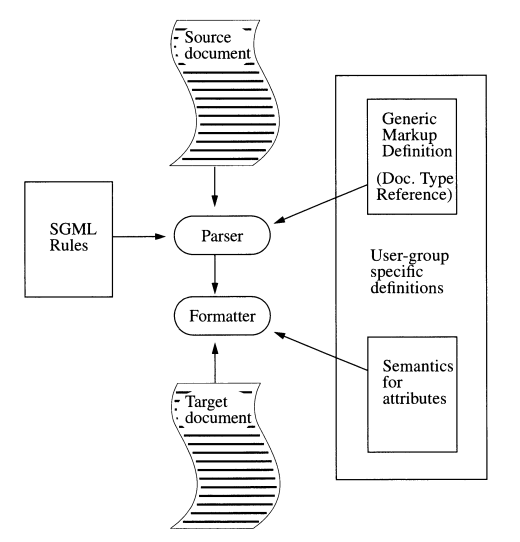
\includegraphics[width=0.7\textwidth]{sgml-doc-processing}
	\caption{SGML document processing, from information to representation.}{\label{fig:sgml-doc-processing}}
\end{figure}
%--------------------------Figure end -------------------

The handling process for an SGML document shown in Figure {\ref{fig:sgml-doc-processing}} splits the processing job into two processes:
\begin{itemize}
	\item The \textit{formatter} knows the meaning of the tags, and uses these tags to produce a formatted document. 
	
	\item The \textit{parser} uses the tags contained in the document in combination with the appropriate document type.
\end{itemize}

Tags can be used to define the structure of a document, which normally includes the association of some parts of the layout. It is based on the common context between the creator of the document and the formatting process, but not defined by SGML. There are various tag categories:

\begin{itemize}
	\item \textit{Descriptive markup tags} describe the actual structure in the following form:
	
\begin{lstlisting}[language=xml, frame=single]
<start-tag> or alternatively <end-tag>
\end{lstlisting}

One example is the definition of the beginning of a paragraph:
\begin{lstlisting}[language=xml, frame=single]
<paragraph> The text of this paragraph begins here ...
\end{lstlisting}

\item An \textit{entity reference} points to another element, which then replaces the entity reference. This could also be interpreted as an abbreviation, which is later overwritten by copying the actual content in its place. The following example shows entity reference in a mathematical context:

\[\mathtt{\&square \: x ... should\: be\: x^2}\]




\item The \textit{markup declarations} define the elements to which an entity reference refers. In our example of squaring a variable $ x $, square is defined as:
\begin{lstlisting}[frame=single]
	<!ELEMENT square (...)>
\end{lstlisting}

A markup declaration can also be used to define rules for the structure (classes). The following example defines the structure of an article \textit{paper}:
	
\begin{lstlisting}[frame=single]
<!ELEMENT paper (preamble, body, postamble)>
<!ELEMENT preamble (title, author, side)>
<!ELEMENT title (#CDATA)> -- character data
<!ELEMENT body (...) >
\end{lstlisting}

\item \textit{Processing Instructions} are used to embed instructions for other programs into a piece of text, e.\ g.\ , instructions for the formatter. Processing instructions can also be used to insert various media, e.\ g.\ , images and video.
\end{itemize}

SGML uses a grammar for tags to define a syntax that has to be observed. It does not define the meaning of these tags.

Figure {\ref{fig:sgml-doc-arch}} shows the information or document architecture of SGML. Using its tags, SGML has a representation model. \textit{Objects}, \textit{classes}, and \textit{inheritance} can be used to define the structure.


%%%%%%%%%%%%%%%%%%%%%%%%%%%%%%%%%%%%%%%%%
%										%
%				FIGURE				   	%
%										%
%%%%%%%%%%%%%%%%%%%%%%%%%%%%%%%%%%%%%%%%%
\begin{figure}[ht!]
	\centering
	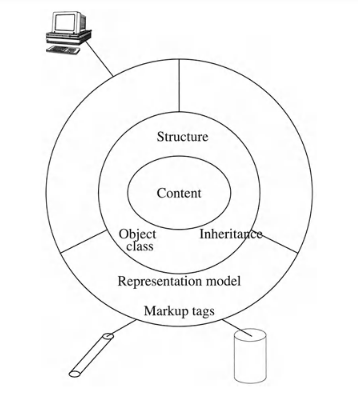
\includegraphics[width=0.7\textwidth]{sgml-doc-arch}
	\caption{The SGML document architecture focuses on the representation model.}{\label{fig:sgml-doc-arch}}
\end{figure}
%--------------------------Figure end -------------------

\subsubsection*{SGML and Multimedia}
\begin{multicols}{2}
	\begin{itemize}
		\item SGML standard supports multimedia data only in the form of images. 
		\item An image is embedded into an SGML document in CGM (\textit{Computer Graphics Metafile}) form. 
		\item The standard does not include specifications or recommendations for other media.
	\end{itemize}
\end{multicols}


\begin{lstlisting}[frame=single]
	<!ATTLIST video 	id 		ID #IMPLIED>
	<!ATTLIST video 	synch 	synch #IMPLIED>
	<!ELEMENT video 	(audio, movpic)>
	<!ELEMENT audio 	(#NDATA)) -- non-text media
	<!ELEMENT movpic 	(#NDATA)) -- non-text media
	...
	<!ELEMENT story 	(preamble, body, postamble)) :
\end{lstlisting}

\verb|#NDATA| can be used to set a reference that points to specific data. This data is normally external, i.\ e.\ , stored in a separate file. The above example shows a video definition, consisting of audio and motion pictures.



\subsection[ODA]{Document Architecture ODA}
The \textit{Open Document Architecture (ODA)} was initially called the \textit{Office Document Architecture} because it supports mostly office-oriented applications. The main goal of this document architecture is to support the exchange, processing and presentation of documents in open systems.

\subsection*{ODA}
\begin{itemize}
\item The main property of ODA is the distinction among \textit{content}, \textit{logical} structure and \textit{layout} structure. 
\item This is in contrast to SGML where only a logical structure and the contents are defined. 
\item ODA also defines semantics. 
\end{itemize}
Figure {\ref{fig:oda}} shows these three aspects linked to a document. One can imagine these aspects as three orthogonal views of the same document. Each of these views represent one aspect, together we get the actual document.

%%%%%%%%%%%%%%%%%%%%%%%%%%%%%%%%%%%%%%%%%
%										%
%				FIGURE				   	%
%										%
%%%%%%%%%%%%%%%%%%%%%%%%%%%%%%%%%%%%%%%%%
\begin{figure}[hpb]
	\centering
	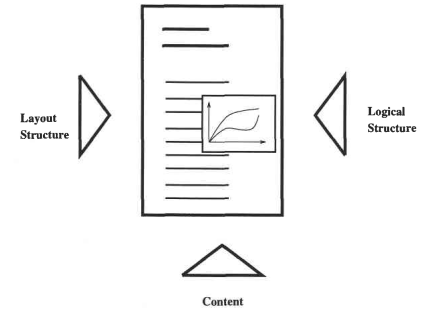
\includegraphics[width=0.8\textwidth]{oda}
	\caption{ODA: Content, layout and logical view.}{\label{fig:oda}}
\end{figure}
%--------------------------Figure end -------------------


\begin{multicols}{2}
	\subsubsection*{Content Portions}
	\begin{itemize}
		\item The content of the document consists of \textit{Content Portions}. 
		\item These can be manipulated according to the corresponding medium.
		\item A content architecture describes for each medium:  
		\begin{itemize}
			\item the specification of the elements
			\item the possible access functions and
			\item the data coding
		\end{itemize}
		\item Individual elements are the Logical Data Units (LDUs), which are determined for each medium. 
		\item The access functions serve for the manipulation of individual elements. 
		\item The coding of the data determines the mapping with respect to bits and bytes.
		\item ODA has content architectures for media text, geometrical graphics and raster graphics.
	\end{itemize}
\end{multicols}



\subsubsection*{Layout Structure and Logical Structure}

The structure and presentation models describe — according to the information architecture — the cooperation of information units. These kinds of meta information distinguish layout and logical structure.

\subsubsection*{Layout Structure}
\begin{multicols}{2}
	\begin{itemize}
		\item The \textit{layout structure} specifies mainly the representation of a document. 
		\item It is related to a two-dimensional representation with respect to a screen or paper. 
		\item The presentation model is a tree. 
		\item Using \textit{frames} the position and size of individual layout elements is established. 
		\item For example, the page size and type style are also determined.
	\end{itemize}
\end{multicols}

\subsubsection*{Logical Structure}
\begin{multicols}{2}
	\begin{itemize}
		\item The \textit{logical structure} includes the partitioning of the content. 
		\item Here, paragraphs and individual headings are specified according to the tree structure. 
	\end{itemize}
\end{multicols}
		

%Lists with their entries are defined (example) as:

%\begin{verbatim}
%	paper = preamble body postamble
%	body = chapter 1, chapter 2
%	chapter 1 = heading, paragraph ... picture ...
%	chapter 2 = heading paragraph picture paragraph
%\end{verbatim}
%The fundamental descriptive means of the structural and presentational models
%are linked to the individual nodes which build a document. The document is seen
%as a tree. Each node (also a document) is a constituent) or an object. It consists of
%a set of attributes, which represent the properties of the nodes. A node itself
%includes a concrete value or it defines relations between other nodes. The
%simplified distinction is between the editing, formatting (Document Layout
%Process and Content Layout Process) and actual presentation (Imaging Process).
%\begin{itemize}
%	\item A \textit{formatted document} includes the specific layout structure, and
%	eventually the generic layout structure. It can be printed directly or
%	displayed, but it cannot be changed.
%	
%	\item A \textit{processable document} consists of the specific logical structure, eventually
%	the generic logical structure, and later of the generic layout structure. The
%	document cannot be printed directly or displayed. Change of content is
%	possible.
%	
%	\item A \textit{formatted processable} document is a mixed form. It can be printed,
%	displayed and the content can be changed.
%\end{itemize}

\subsection{MHEG}
The committee ISO/IEC JTC1/SC29 (\textit{Coding of Audio, Picture, Multimedia and Hypermedia Information}) works on the standardization of the exchange format for multimedia systems. The actual standards are developed at the international level in three working groups cooperating with research and industry. The results of the working groups: the \textit{Joint Photographic Expert Group (JPEG)} and the \textit{Motion Picture Expert Group (MPEG)} are of special importance in the area of multimedia systems.

In a multimedia presentation, the contents, in the form of individual information objects, are described with the help of the above named standards. The structure is specified first through timely spatial relations between the information objects. The standard of this structure description is the subject of the working group WG12, which is known as the \textit{Multimedia and Hypermedia Information Coding Expert Group (MHEG)}. The name of the developed standard is officially called \textit{Information Technology — Coding of Multimedia and Hypermedia Information (MHEG)}. 


\subsubsection{Example of an Interactive Multimedia Presentation}
Figure {\ref{fig:timing-diagram-multimedia}} presents a time diagram of an interactive multimedia presentation. The presentation starts with some music. As soon as the voice of a news-speaker is heard in the audio sequence, a graphic should appear on the screen for a couple of seconds. After the graphic disappears, the viewer carefully reads a text. After the text presentation ends, a Stop button appears on the screen. With this button the user can abort the audio sequence. Now, using a displayed input field, the user enters the title of a desired video sequence. These video data are displayed immediately after the modification.

%timing-diagram-multimedia
%%%%%%%%%%%%%%%%%%%%%%%%%%%%%%%%%%%%%%%%%
%										%
%				FIGURE				   	%
%										%
%%%%%%%%%%%%%%%%%%%%%%%%%%%%%%%%%%%%%%%%%
\begin{figure}[ht!]
	\centering
	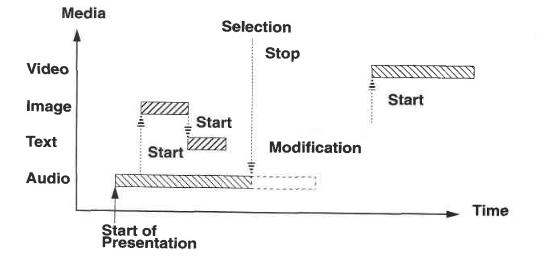
\includegraphics[width=0.8\textwidth]{timing-diagram-multimedia}
	\caption{The timing diagram of an interactive presentation.}{\label{fig:timing-diagram-multimedia}}
\end{figure}
%--------------------------Figure end -------------------


\begin{multicols}{2}
	\paragraph*{Content}
	\begin{itemize}
		\item A presentation consists of a sequence of information representations. 
		\item For the representation of this information, media with very different properties are available. 
		\item Because of later \textit{reuse}, it is useful to capture each information	as an individual object. 
		\item The contents in our example are: 
		\begin{itemize}
			\item the video sequence, 
			\item the audio sequence, 
			\item the graphics, and 
			\item the text.
		\end{itemize}
	\end{itemize}
\end{multicols}


\begin{multicols}{2}
	\paragraph*{Behavior}
	\begin{itemize}
	\item The notion \textit{behavior} means all information which specifies the representation of the contents as well as defines the run of the presentation. 
	\item The first part is controlled by the actions \textit{start}, \textit{set volume}, \textit{set position}, etc.
	\item The last part is generated by the definition of timely, spatial and conditional links between individual elements. 
	\item If the state of the content's presentation changes, then this may result in further commands on other objects (e.\ g.\ , the deletion of the graphic causes the display of the text). 
	\item Another possibility, how the behavior of a presentation can be determined, is when external programs or functions (script) are called.
	\end{itemize}
\end{multicols}




\begin{multicols}{2}
	\paragraph*{User Interaction}
	\begin{itemize}
		\item In the discussed scenario, the running animation could be aborted by a corresponding user interaction. 
		\item There can be two kinds of user interactions.
		\begin{itemize}
			\item \textit{simple selection}, which controls the run of the presentation through a pre-specified choice (e.\ g.\ , push the Stop button). 
			\item complex \textit{modification} which gives the user the possibility to enter data during the run of the presentation (e.\ g.\, editing of a	data input field).
		\end{itemize}
	\end{itemize}
\end{multicols}



\begin{multicols}{2}
	\paragraph*{Container}
	\begin{itemize}
		\item Merging together several elements as discussed above, a presentation,	which progresses in time, can be achieved. 
		\item To be able to exchange this presentation between the involved systems, a \textit{composite} element is necessary. 
		\item This element is comparable to a container. 
		\item It links together all the	objects into a unit. 
		\item With respect to hypertext/ hypermedia documents, such	containers can be ordered to a complex structure, if they are linked together through so-called hypertext pointers.
	\end{itemize}
\end{multicols}


\subsubsection{MHEG Class Hierarchy}
%mheg-class-hierarchy

Figure {\ref{fig:mheg-class-hierarchy} summarizes the individual elements in the MHEG class hierarchy in the form of a tree. 
\begin{multicols}{2}
	\begin{itemize}
		\item Instances can be created from all leaves(roman printed classes). 
		\item All internal nodes, including the root (\textit{italic} printed classes), are abstract classes, i.\ e.\ , no instances can be generated from them. 
		\item The leaves inherit some attributes from the root of the tree as an abstract basic class. 
		\item The internal nodes do not include any	further functions. 
		\item Their task is to unify individual classes into meaningful groups.
		\item The \textbf{action}, the \textbf{link} and the \textbf{script} classes are grouped under the \textbf{behavior} class, which defines the behavior in a presentation. 
		\item The \textbf{interaction} class includes the user interaction, which is again modeled through the \textbf{selection} and \textbf{modification} class. 
		\item All the classes together with the \textbf{content} and \textbf{composite} classes specify the individual components in the presentation and determine the \textbf{component} class. 
		\item Some properties of the particular MHEG engine can be queried by the \textbf{descriptor} class
		\item The \textbf{macro}	class serves as the simplification of the access, respectively reuse of objects. Both classes play a minor role.
	\end{itemize}
\end{multicols}


%%%%%%%%%%%%%%%%%%%%%%%%%%%%%%%%%%%%%%%%%
%										%
%				FIGURE				   	%
%										%
%%%%%%%%%%%%%%%%%%%%%%%%%%%%%%%%%%%%%%%%%
\begin{figure}[ht!]
	\centering
	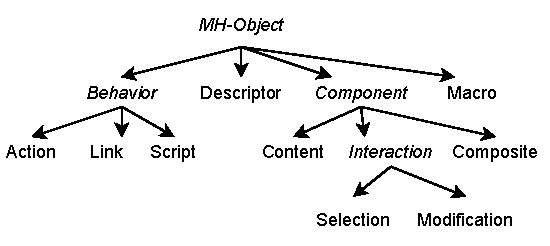
\includegraphics[width=0.8\textwidth]{mheg-class-hierarchy}
	\caption{Class hierarchy of MHEG objects.}{\label{fig:mheg-class-hierarchy}}
\end{figure}
%--------------------------Figure end -------------------

\paragraph*{MH-Object Class}
The abstract MH-Object Class inherits both data structures \textit{MHEG identifier} and \textit{Descriptor}.

\begin{multicols}{2}
	\begin{itemize}
		\item MHEG identifier consists of the attributes \textit{MHEG identifier} and \textit{Object Number} and it serves as the addressing of MHEG objects. 
		\item The first attribute identifies a specific application. 
		\item The \textit{Object Number} is a number which is defined only within the application. 
		\item The data structure \textit{Descriptor} provides the possibility to characterize more precisely each MHEG object through a number of optional attributes. 
		\item For example, this can become meaningful if a presentation is decomposed into individual objects and the individual MHEG objects are stored in a database. 
		\item Any author, supported by proper search functions, can reuse existing MHEG objects.		
	\end{itemize}
\end{multicols}
